
\section{Abstract}
Das Teamprojekt DeepRain bestehend aus fünf Studierenden aus den Masterstudiengängen MSI und BIT startete im Wintersemester 18/19 an der HTWG Konstanz. Das Ziel ist innerhalb eines Jahres einen lauffähigen Algorithmus auf Github (thgnaedi/DeepRain) zur Verfügung zu stellen. Dieser soll mit Hilfe von Deep Learning in der Lage sein, das Wetter in Konstanz, bzw. den Niederschlag im Zeitraum von einer Stunde vorherzusagen. Betreut wird das Projekt während dem Jahr von Prof. Oliver Duerr. 
Eine möglichst korrekte Wettervorhersage hat viele, gut ersichtliche Vorteile. Das fängt bei dem recht alltäglichen Verlassen des Hauses mit- oder eben ohne den Regenschirm an, je nach Wettervorhersage, und dem Vertrauen darauf, dass diese Vorhersage auch stimmt und man nicht nass wird. Vorhersagen mit Deep Learning-Unterstützung finden auch eine sehr wichtige Verwendung in der Katastrophenvorhersage und dem Katastrophenmanagement (vgl. \cite[S. 763]{Hanif.2019}). Bei der Energieversorgung spielt es auch eine wichtige Rolle, zum Beispiel bei der Planung der Auslastung von Solar-Panels (vgl. \cite[S. 2]{AndreGensleret.al..}). Die Wettervorhersage an sich wird jedoch bisher noch nicht mit Deep Learning-Techniken generiert, dies ist erst ab diesem Jahr bei einigen Anbietern angedacht (vgl. \cite{ChristophFrohlich.2019}. 
\begin{figure}[ht]
\centering
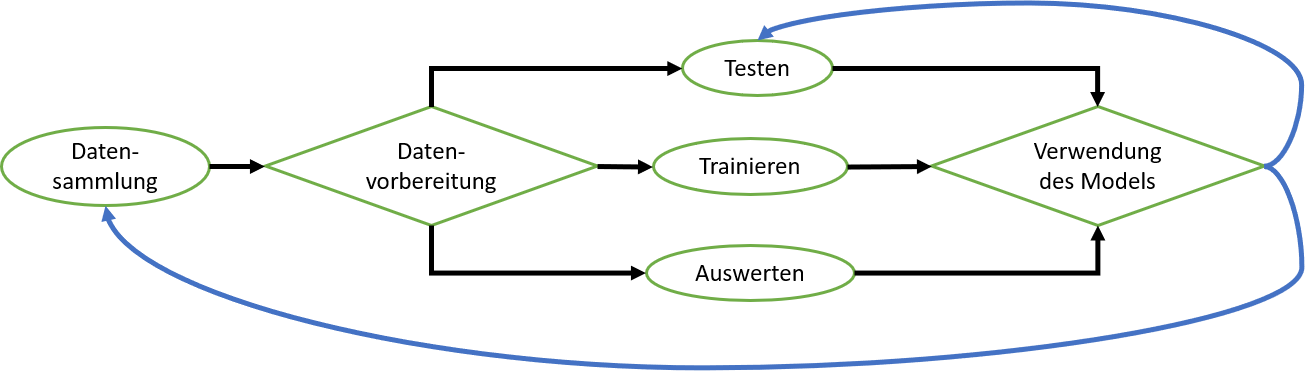
\includegraphics[width=\linewidth]{pics/Deep_learning_prozess}
\caption{Wichtige Schritte im Prozess des DeepRain-Projekts, Eigene Darstellung}
\label{fig:deepLearningProcess}
\end{figure}
Im Rahmen des Teamprojekts stand zu Beginn ein Eindenken in die Prozesse des Maschine-Learnings an und bereits vorhandene Forschung zu recherchieren. Dann stand erstmal die Datenbeschaffung im Vordergrund und die Qualitätsbewertung der vorhandenen Daten. Später im Projekt ging es dann an die Entwicklung des Algorithmus. Der Verlauf dieser Arbeit lehnt sich diesen auch in \ref{fig:deepLearningProcess} dargestellten Prozess an. 

\subsection{Deep Learning}
Deep Learning basiert auf der Optimierung von künstlichen neuronalen Netzen (KNN) und ist eine Weiterentwicklung von Maschine Learning (vgl. \cite[S. 1]{Georgevici.2019}). Ziel von neuronalen Netzen ist es die Aufgabenlösung in ähnlicher Weise zu ermöglichen wie es im menschlichen Gehirn geschieht. Kern ist hier das “Lernen” und das Lösen von Problemen. Neuronale Netze haben sich vor allem wegen ihrer Fähigkeit der Verarbeitung von ständig wachsenden Datenmengen und -komplexität etabliert (vgl. \cite[S. 373]{Welsch.2018}). In einem künstlichen neuralen Netzwerk müssen nicht im Vorhinein Vermutungen über Zusammenhänge festgelegt werden sondern diese werden im Lernprozess vom Netz ermittelt (vgl. \cite[S. 581]{Backhaus.2018b}). Ein Neurales Netz ist 
so aufgebaut, dass es einen bekannten Input gibt, der dann durch einen Hidden-Layer, das aus Neuronen besteht läuft in dem das Lernen stattfindet und ein Output generiert wird. Hier können einige Variablen, die den Output 
beeinflussen, festgelegt werden. 
Die Neuronen modifizieren dabei die Daten und leiten diese dann weiter (vgl. \cite[S. 373]{Welsch.2018}). Es kann sich auch zwischen einer biologischen oder einer technischen Simulation von Neuronen entschieden werden (vgl. \cite{https:www.facebook.comspektrumverlag.04.12.2014}). Die technische Simulation wird zur Datenverarbeitung und Mustererkennung meist bevorzugt (vgl. \cite{https:www.facebook.comspektrumverlag.04.12.2014}). Dieser Zusammenhang wird in \ref{fig:NeuralVsDeepNeural} dargestellt. 
In dieser Abbildung wird auch ersichtlich, wodurch sich ein Deep Neural Network von einem neuralen Netz unterscheidet. Hier wird gleich mit mehreren Hidden-Layers, die hintereinander liegen gearbeitet. Die Verwendung mehrere Hidden-Layers führt dabei laut (\cite[S. 581]{Backhaus.2018b}) zu erfahrungsgemäß korrekteren Lernergebnissen. Das „Lernen“ hängt dann vom Grad der Aktivierung der einzelnen Neuronen ab. Dieser wird durch die bisherigen Ergebnisse durch eine ermittelte Gewichtung einzelner Neuronen bestimmt. Diese Gewichtung wird im Verlauf des Lernens im Netz im besten Fall immer mehr optimiert (vgl. \cite[S. 586]{Backhaus.2018b}).
\begin{figure}[ht]
\centering
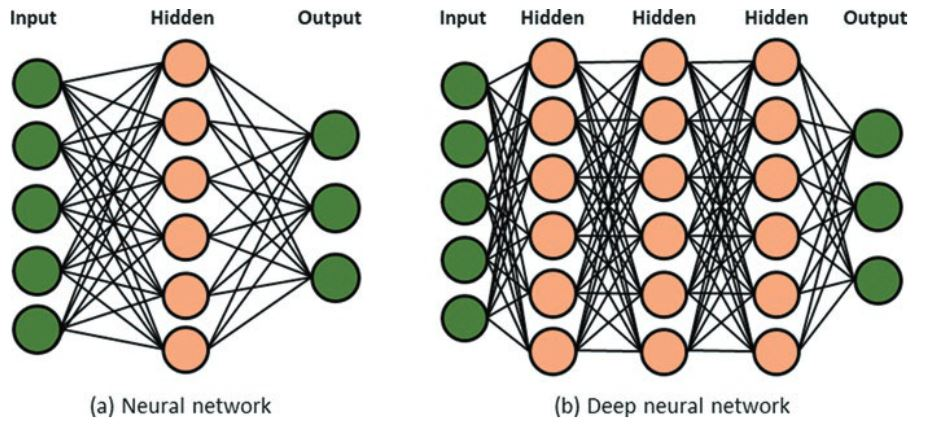
\includegraphics[width=\linewidth]{pics/ANN_for_deep_learning_P35}
\caption{Unterscheidung Neurales Netzwerk und Deep-neurales Netzwerk, Quelle: ANN for deep learning (Akerkar 2019, S. 35)}
\label{fig:NeuralVsDeepNeural}
\end{figure}
In unserem Projekt soll mithilfe von neuronalen Netzen das Lernen aus bisherigen Wetterdaten ermöglicht werden, sodass dann eine möglichst korrekte Wettervorhersage durch das Netz für eine Stunde in die Zukunft generiert wird.

\subsection{State-of-the-art Wettervorhersage mit Deep Learning}

Über Deep Learning und auch Machine-Learning, Neuro- und Lin"-gu"-al-Pro"-gram"-ming findet sich einige Literatur. Jedoch steht die Nutzung zur Wettervorhersage noch am Anfang (vgl. \cite{ChristophFrohlich.2019}). Dies wird auch dadurch unterstützt, dass auf GitHub zum aktuellen Stand (August 2019) gerade einmal eine Handvoll Repositories zum Thema Deep Learning und Wettervorhersage existiert. Verfahren werden verbessert, die Lernverfahren den Menschlichen Lernen immer ähnlicher, die Entwicklung ist stetig steigend und wie oben erwähnt sind noch viele Bereiche wie u.a. die Wettervorhersage  ergründbar (\cite[S. 103]{Wick.2017}). Im Bereich der Wettervorhersage bietet sich in Anlehnung an Abbildung 3 in den meisten Fällen das Supervised Learning, da eine möglichst genaue Vorhersage das Ziel ist. Aber auch das  nicht-überwachte Lernen kann interessante Schlüsse zulassen, um eventuell unbekannte Muster zu finden (vgl. \cite[S. 371]{Welsch.2018}). 
